\documentclass[aspectratio=169,11pt]{beamer}

% -------------------------------------------------
% Theme and packages
% -------------------------------------------------
\usetheme{Madrid}
\usecolortheme{default}

\usepackage[utf8]{inputenc}
\usepackage[T1]{fontenc}
\usepackage{lmodern}
\usepackage{graphicx}
\usepackage{booktabs}
\usepackage{array}
\usepackage{xcolor}
\usepackage{tikz}
\usepackage{amsmath}
\usepackage{multicol}
\usepackage{ragged2e}

% -------------------------------------------------
% Clean academic color palette
% -------------------------------------------------
\definecolor{MitoNavy}{HTML}{172033}
\definecolor{MitoBlue}{HTML}{2F5D8C}
\definecolor{MitoSlate}{HTML}{475569}
\definecolor{MitoGray}{HTML}{6B7280}
\definecolor{MitoLightGray}{HTML}{F3F4F6}
\definecolor{MitoSoftBlue}{HTML}{EAF2F8}
\definecolor{MitoGreen}{HTML}{2E7D32}
\definecolor{MitoRed}{HTML}{B91C1C}

% -------------------------------------------------
% Beamer styling
% -------------------------------------------------
\setbeamercolor{normal text}{fg=MitoNavy,bg=white}
\setbeamercolor{frametitle}{fg=white,bg=MitoNavy}
\setbeamercolor{title}{fg=MitoNavy}
\setbeamercolor{subtitle}{fg=MitoSlate}
\setbeamercolor{author}{fg=MitoSlate}
\setbeamercolor{institute}{fg=MitoSlate}
\setbeamercolor{date}{fg=MitoSlate}
\setbeamercolor{structure}{fg=MitoBlue}

\setbeamercolor{block title}{fg=white,bg=MitoBlue}
\setbeamercolor{block body}{fg=MitoNavy,bg=MitoSoftBlue}

\setbeamertemplate{navigation symbols}{}
\setbeamertemplate{footline}[frame number]

\setbeamertemplate{itemize item}{\color{MitoBlue}$\blacktriangleright$}
\setbeamertemplate{itemize subitem}{\color{MitoBlue}$\circ$}

% -------------------------------------------------
% Typography helpers
% -------------------------------------------------
\newcommand{\keyword}[1]{\textcolor{MitoBlue}{\textbf{#1}}}

\newcommand{\metriccard}[3]{
\begin{block}{#1}
\centering
{\Large \textbf{#2}}\\
\vspace{0.2em}
{\small #3}
\end{block}
}

\newcommand{\sectiondivider}[2]{
{
\setbeamertemplate{footline}{}
\begin{frame}[plain]
\begin{tikzpicture}[remember picture,overlay]
    \fill[MitoNavy] (current page.south west) rectangle (current page.north east);
    \node[align=center,text=white] at (current page.center) {
        {\huge \textbf{#1}}\\[0.8em]
        {\large #2}
    };
\end{tikzpicture}
\end{frame}
}
}

% -------------------------------------------------
% Title information
% -------------------------------------------------
\title[MitoChime]{MitoChime}
\subtitle{A Machine Learning Pipeline for Detecting PCR-Induced Chimeric Reads in Mitochondrial Illumina Data}

\author{
Duranne Duran \and
Yvonne Lin \and
Daniella Pailden
}

\institute{
University of the Philippines Visayas\\
Division of Physical Sciences and Mathematics
}

\date{Special Problem Defense}

\newcommand{\presenters}{Duranne Duran \quad $\cdot$ \quad Yvonne Lin \quad $\cdot$ \quad Daniella Pailden}

\begin{document}

% -------------------------------------------------
% Slide 1: Title
% -------------------------------------------------
{
\setbeamertemplate{footline}{}
\begin{frame}[plain]
\vspace{1.1cm}

\begin{center}
{\Large \textcolor{MitoSlate}{Special Problem Defense}}\\[1.2em]

{\Huge \textbf{MitoChime}}\\[0.6em]

{\large A Machine Learning Pipeline for Detecting PCR-Induced}\\
{\large Chimeric Reads in Mitochondrial Illumina Data}\\[1.6em]

\rule{0.65\linewidth}{0.5pt}\\[1.2em]

{\normalsize
\presenters
}\\[0.7em]

{\small
University of the Philippines Visayas\\
Division of Physical Sciences and Mathematics
}

\end{center}
\end{frame}
}

% -------------------------------------------------
% Slide 2: Hook
% -------------------------------------------------
\begin{frame}{Opening question: which read is artificial?}

\begin{columns}[T]
\column{0.58\textwidth}
\centering
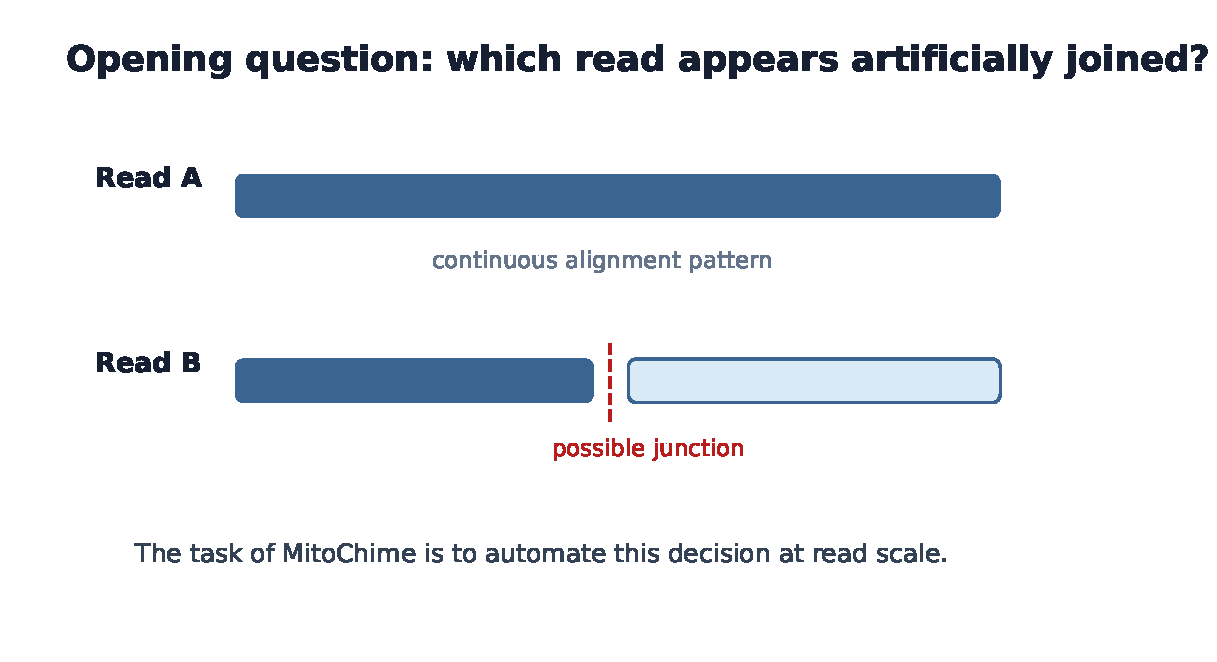
\includegraphics[width=0.92\linewidth]{figures/impostor_reads.pdf}

\column{0.38\textwidth}
\begin{block}{Framing question}
Which read shows evidence of being artificially joined?
\end{block}

\vspace{0.8em}

\begin{itemize}
    \item Sequencing datasets contain thousands of reads.
    \item Manual inspection is not practical.
    \item The goal is automated read-level detection.
\end{itemize}

\end{columns}

\end{frame}

% -------------------------------------------------
% Slide 3: Real-world problem
% -------------------------------------------------
\begin{frame}{Real-world problem}

\begin{columns}
\column{0.48\textwidth}
\centering
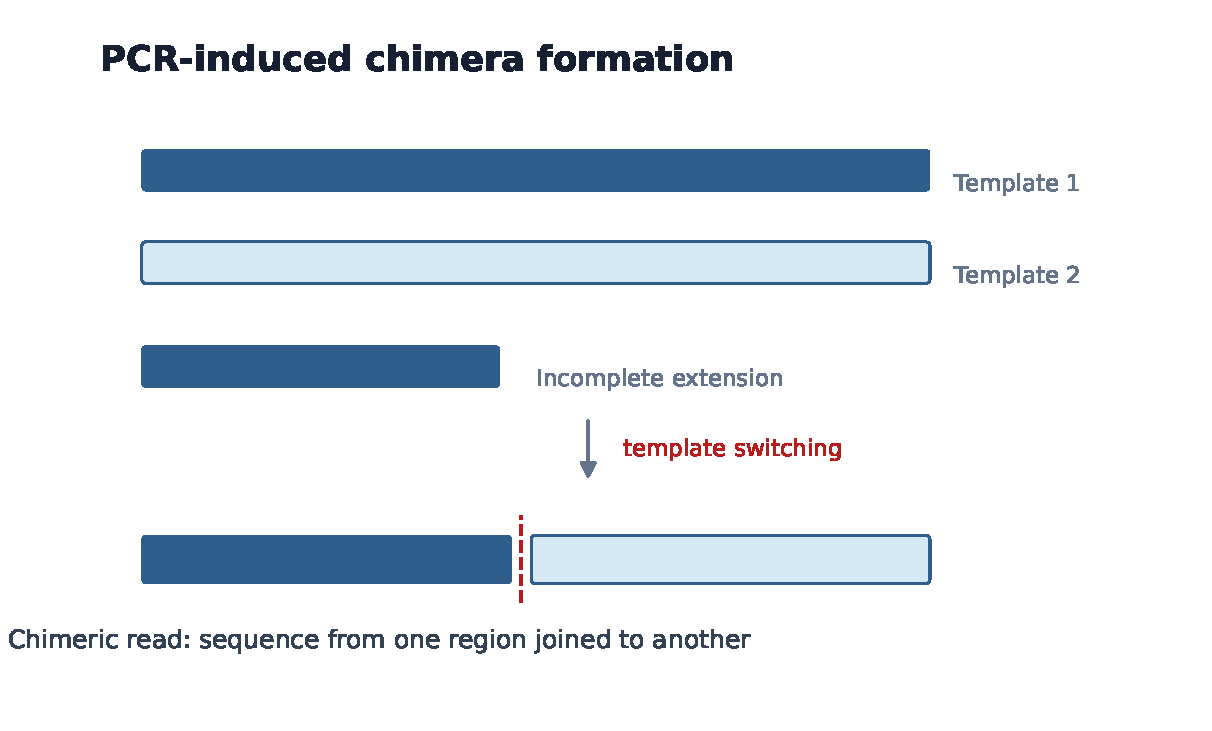
\includegraphics[width=0.92\linewidth]{figures/pcr_chimera.pdf}

\column{0.48\textwidth}
\Large
PCR amplification can produce\\
\keyword{artificial hybrid reads}.\\[0.8em]

\normalsize
These reads may be included in sequencing data and mislead mitochondrial genome assembly.

\vspace{1em}

\begin{block}{Core issue}
Some reads appear valid but do not represent the original mitochondrial sequence.
\end{block}

\end{columns}

\end{frame}

% -------------------------------------------------
% Slide 4: Implications
% -------------------------------------------------
\begin{frame}{Why the problem matters}

\begin{columns}[T]
\column{0.33\textwidth}
\metriccard{Assembly}{Fragmentation}{Contigs may break or branch}

\column{0.33\textwidth}
\metriccard{Analysis}{False signals}{Incorrect junctions may appear}

\column{0.33\textwidth}
\metriccard{Interpretation}{Lower reliability}{Downstream conclusions weaken}
\end{columns}

\vspace{1em}

\begin{center}
\large
For \textit{Sardinella lemuru}, unreliable mitochondrial assemblies may affect fisheries genetics, population structure, and evolutionary analysis.
\end{center}

\end{frame}

% -------------------------------------------------
% Slide 5: Existing approaches
% -------------------------------------------------
\begin{frame}{Existing approaches}

\begin{columns}[T]
\column{0.32\textwidth}
\begin{block}{Reference-based}
Compares query sequences against known non-chimeric references.
\end{block}

\column{0.32\textwidth}
\begin{block}{De novo}
Uses internal dataset patterns such as abundance and similarity.
\end{block}

\column{0.32\textwidth}
\begin{block}{Tool-based}
Includes UCHIME, UCHIME2, DADA2, CATCh, and ChimPipe.
\end{block}
\end{columns}

\vspace{1.2em}

\centering
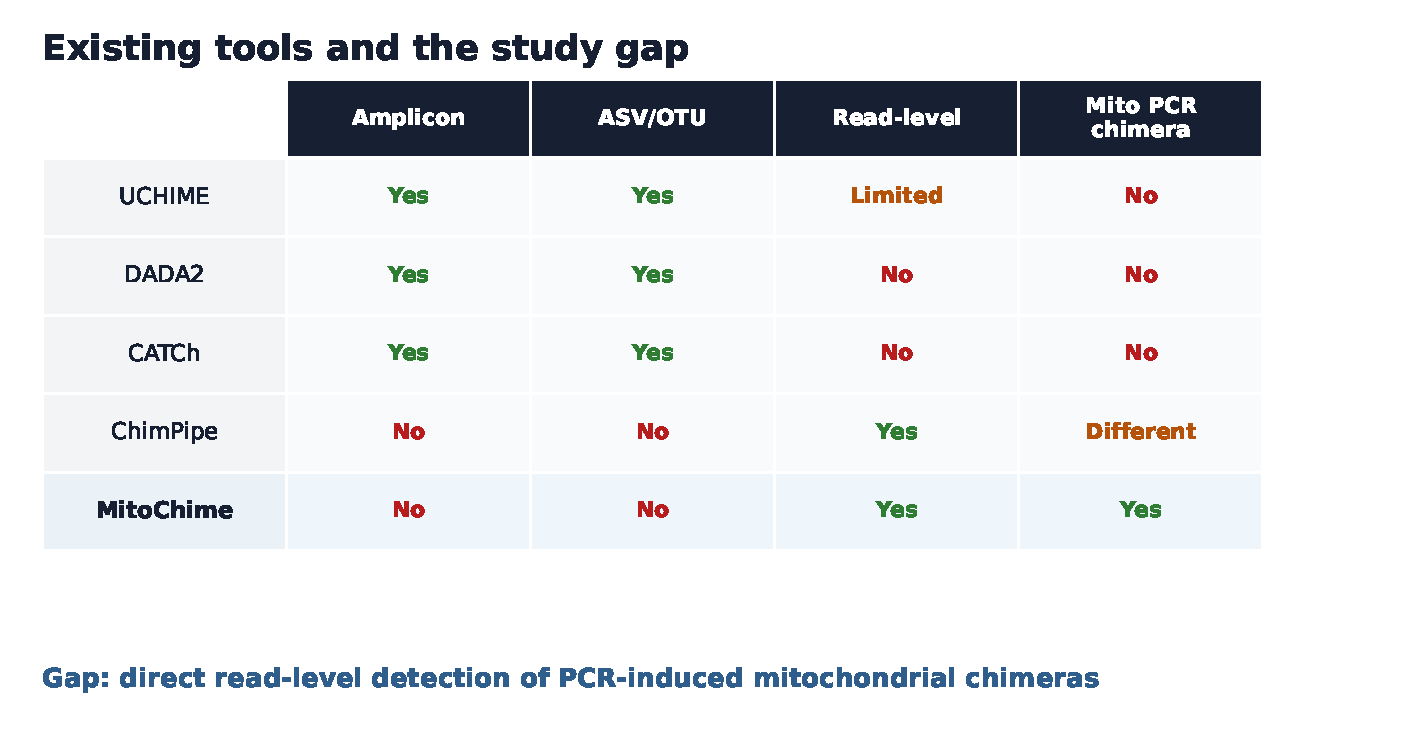
\includegraphics[width=0.76\linewidth]{figures/tool_gap_matrix.pdf}

\end{frame}

% -------------------------------------------------
% Slide 6: Gap
% -------------------------------------------------
\begin{frame}{Research gap}

\Large
Most existing tools were designed for:\\[0.5em]

\normalsize
\begin{itemize}
    \item microbial amplicon or ASV/OTU-level analysis,
    \item reference-based or abundance-based detection,
    \item community-level filtering,
    \item biological chimeras or other sequencing contexts.
\end{itemize}

\vspace{1em}

\begin{block}{Gap addressed by this study}
There is limited support for direct \keyword{read-level detection} of PCR-induced chimeras in single-species mitochondrial Illumina data.
\end{block}

\end{frame}

% -------------------------------------------------
% Slide 7: Study problem
% -------------------------------------------------
\begin{frame}{Study problem}

\begin{center}
\Large
Can machine learning detect PCR-induced chimeric reads\\
\keyword{before mitochondrial genome assembly}?
\end{center}

\vspace{1.5em}

\begin{columns}[T]
\column{0.48\textwidth}
\begin{block}{Input}
Simulated clean and chimeric paired-end Illumina reads from \textit{S. lemuru}
\end{block}

\column{0.48\textwidth}
\begin{block}{Output}
A modular pipeline that predicts and filters suspected chimeric reads
\end{block}
\end{columns}

\end{frame}

% -------------------------------------------------
% Slide 8: Scope and limitations
% -------------------------------------------------
\begin{frame}{Scope and limitations}

\begin{columns}[T]
\column{0.48\textwidth}
\begin{block}{Included}
\begin{itemize}
    \item \textit{Sardinella lemuru}
    \item mitochondrial Illumina reads
    \item PCR-induced chimeras
    \item simulated labelled datasets
\end{itemize}
\end{block}

\column{0.48\textwidth}
\begin{block}{Excluded}
\begin{itemize}
    \item long-read sequencing
    \item NUMTs
    \item naturally occurring chimeras
    \item broad multi-species validation
\end{itemize}
\end{block}
\end{columns}

\vspace{0.9em}
\centering
\large
The study prioritized a focused and controlled evaluation setting.

\end{frame}

% -------------------------------------------------
% Slide 9: Section divider
% -------------------------------------------------
\sectiondivider{Methodology}{From simulated reads to model-based filtering}

% -------------------------------------------------
% Slide 10: Workflow
% -------------------------------------------------
\begin{frame}{MitoChime workflow}

\centering
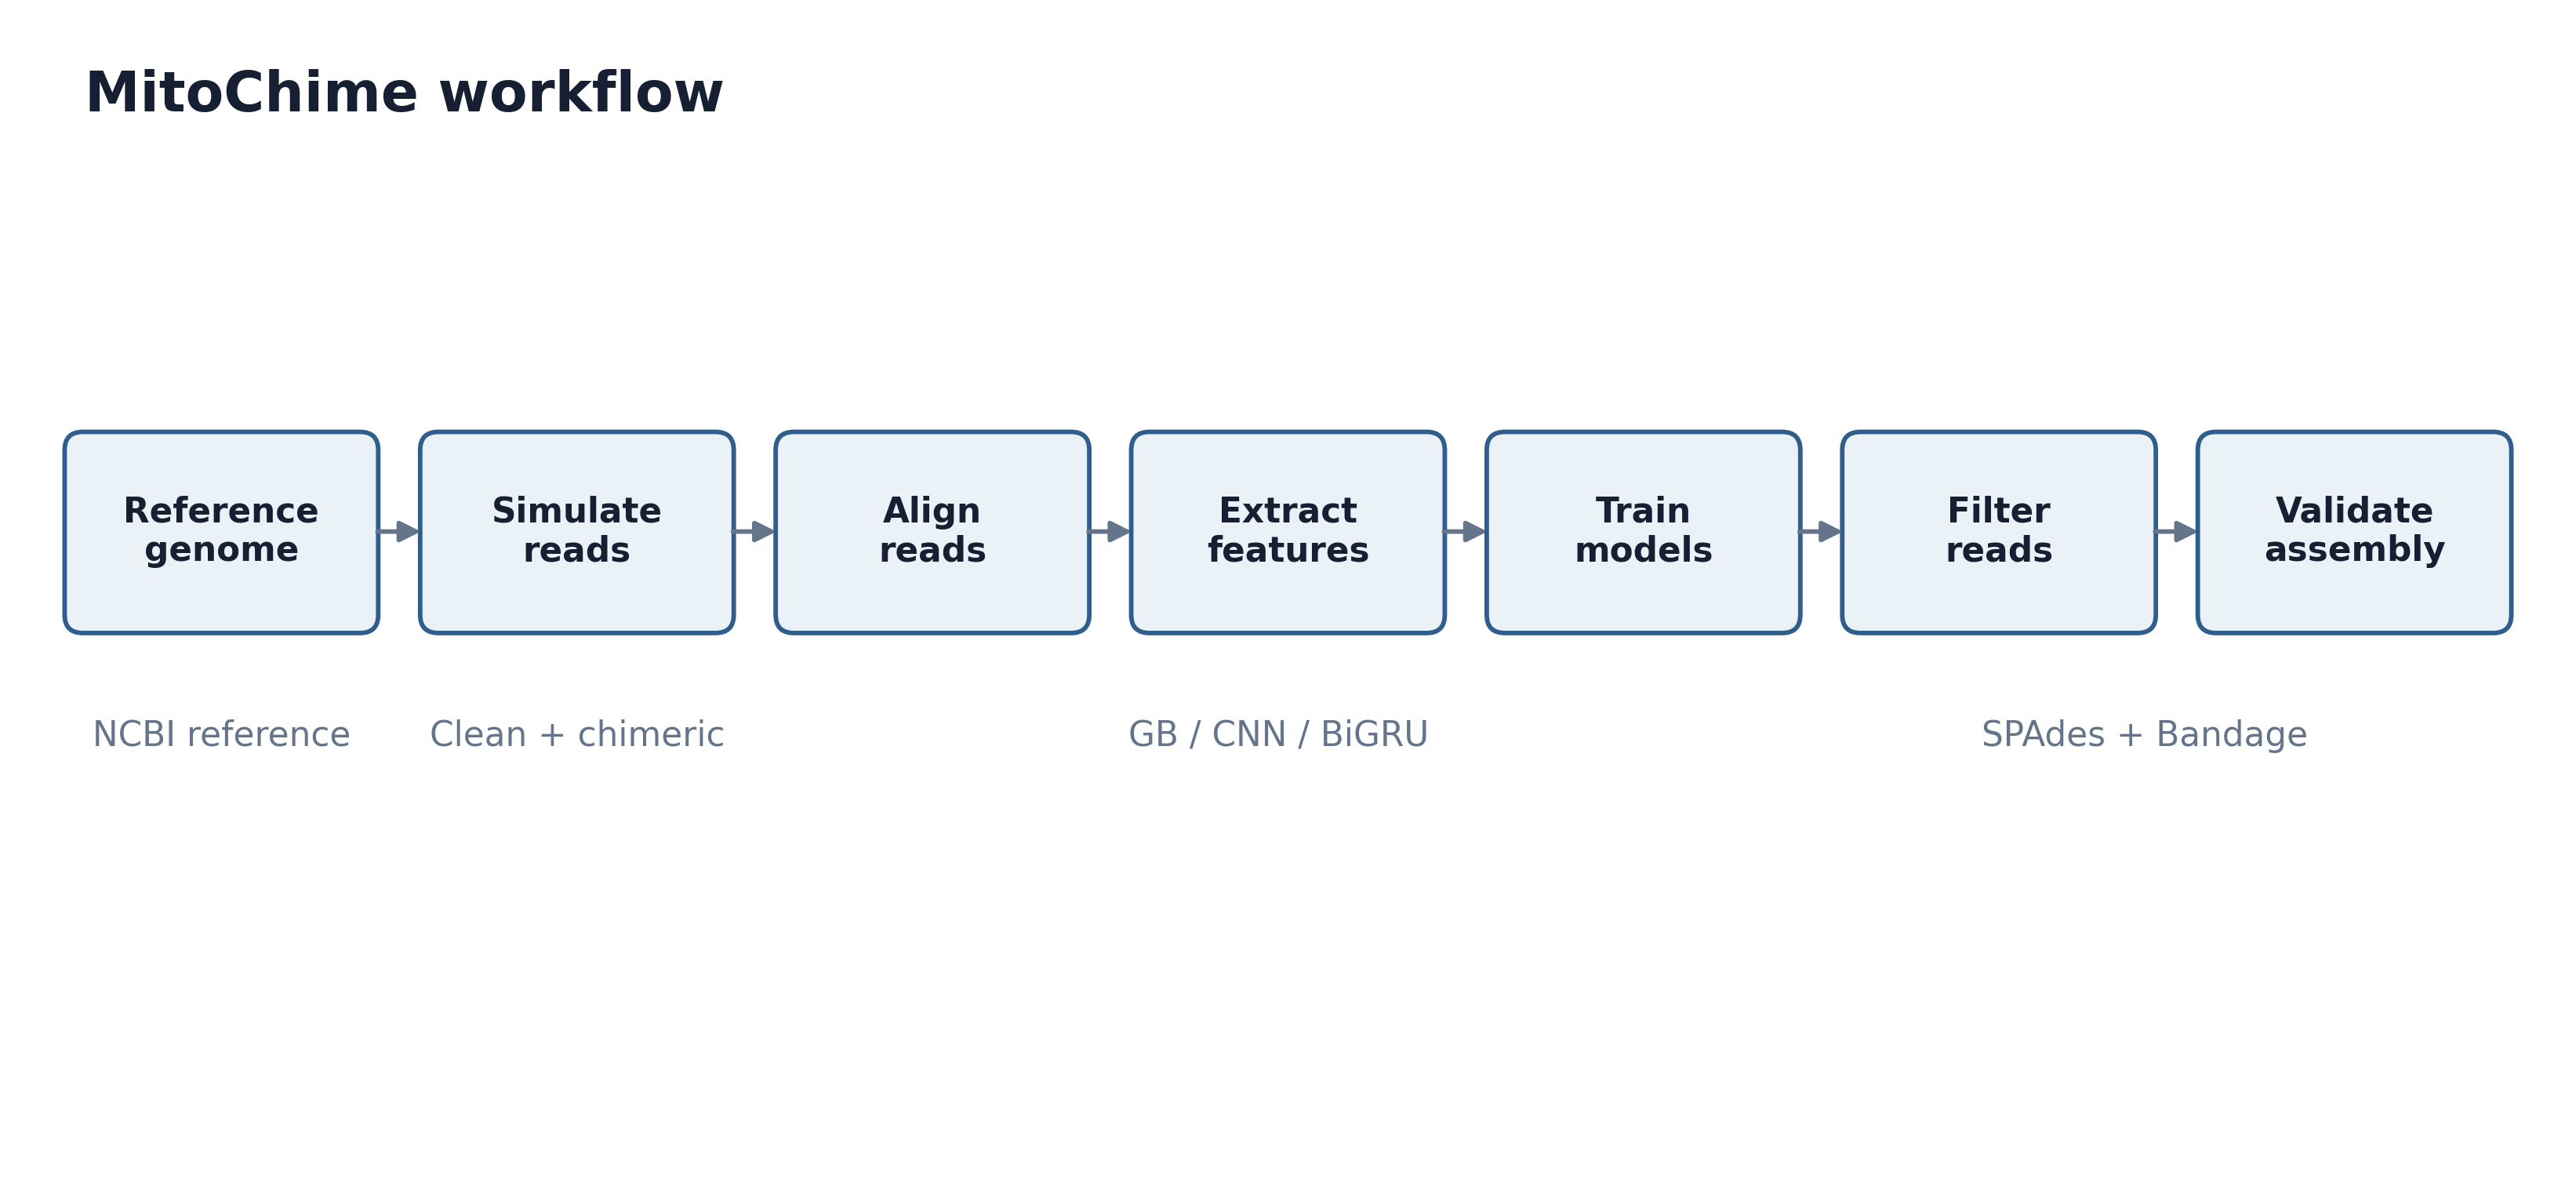
\includegraphics[width=0.70\linewidth]{figures/methodology.png}

\vspace{0.6em}

\begin{block}{Overview}
The workflow generated labelled reads, extracted read-level evidence, trained models, filtered suspected chimeras, and evaluated downstream assembly behavior.
\end{block}

\end{frame}

% -------------------------------------------------
% Slide 11: Data construction
% -------------------------------------------------
\begin{frame}{Data construction}

\begin{columns}[T]
\column{0.48\textwidth}
\begin{block}{Clean reads}
Simulated from the \textit{S. lemuru} mitochondrial reference genome.
\end{block}

\column{0.48\textwidth}
\begin{block}{Chimeric reads}
Generated by joining non-adjacent mitochondrial segments to mimic PCR template switching.
\end{block}
\end{columns}

\vspace{1.2em}

\centering
\large
Labels: \textcolor{MitoGreen}{clean = 0} \quad and \quad \textcolor{MitoRed}{chimeric = 1}

\end{frame}

% -------------------------------------------------
% Slide 12: Feature extraction
% -------------------------------------------------
\begin{frame}{Feature extraction}

\centering
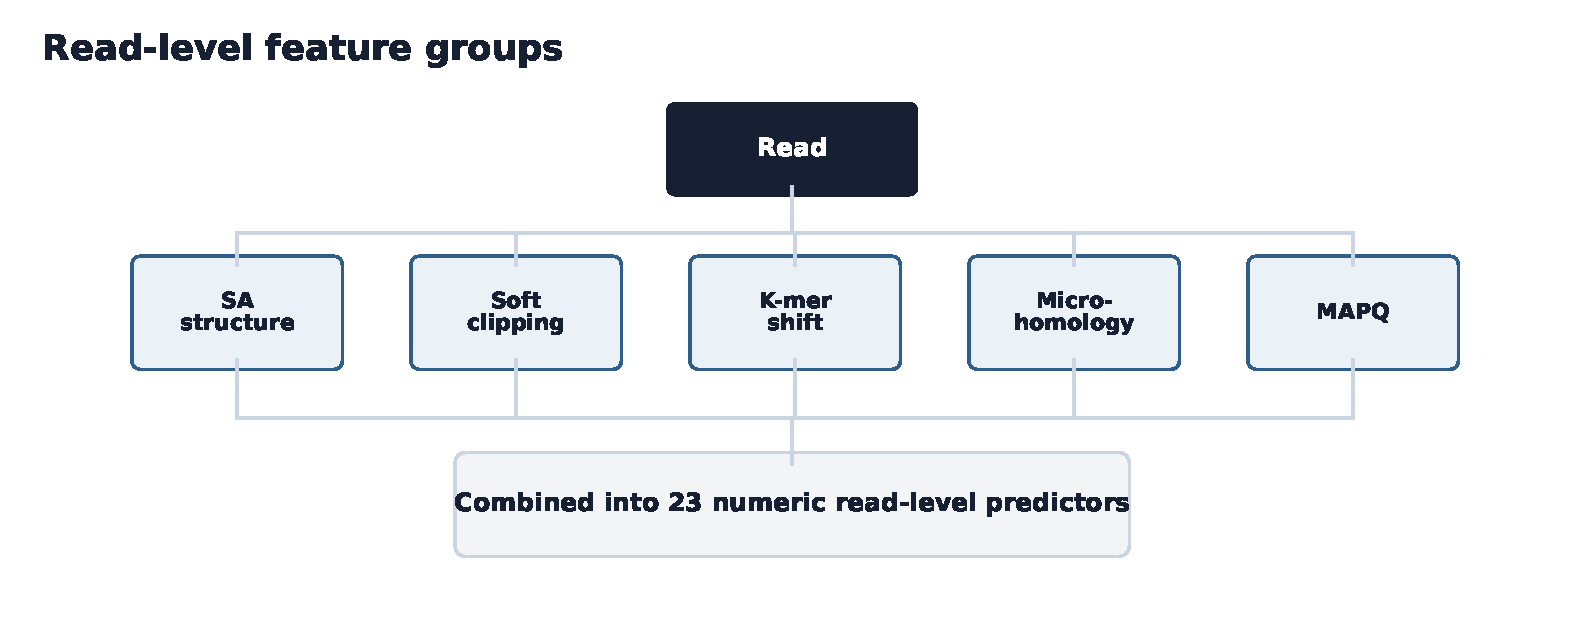
\includegraphics[width=0.80\linewidth]{figures/feature_families.pdf}

\vspace{0.8em}

\begin{columns}[T]
\column{0.2\textwidth}
\centering
\small SA structure

\column{0.2\textwidth}
\centering
\small Soft clipping

\column{0.2\textwidth}
\centering
\small K-mer shift

\column{0.2\textwidth}
\centering
\small Microhomology

\column{0.2\textwidth}
\centering
\small MAPQ
\end{columns}

\vspace{0.8em}

\small
The classical machine learning models used 23 numeric read-level predictors.

\end{frame}

% -------------------------------------------------
% Slide 13: Models
% -------------------------------------------------
\begin{frame}{Models evaluated}

\begin{columns}[T]
\column{0.32\textwidth}
\begin{block}{Gradient Boosting}
Feature-based model using engineered alignment and sequence-derived predictors.
\end{block}

\column{0.32\textwidth}
\begin{block}{1D CNN}
Sequence-based model using one-hot encoded nucleotide reads.
\end{block}

\column{0.32\textwidth}
\begin{block}{BiGRU}
Sequence-based model using ordered k-mer tokens.
\end{block}
\end{columns}

\vspace{1em}

\centering
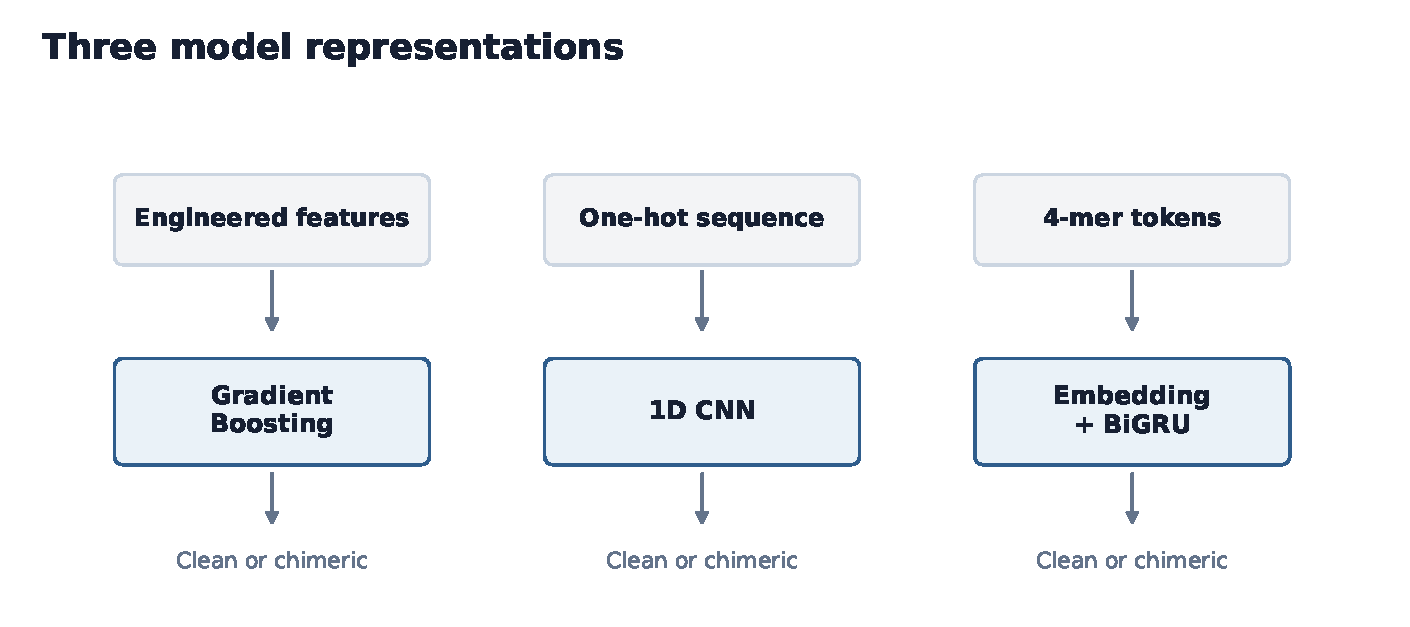
\includegraphics[width=0.72\linewidth]{figures/model_architecture.pdf}

\end{frame}

% -------------------------------------------------
% Slide 14: Evaluation
% -------------------------------------------------
\begin{frame}{Evaluation strategy}

\begin{columns}[T]
\column{0.48\textwidth}
\begin{block}{Read-level evaluation}
\begin{itemize}
    \item Accuracy
    \item Precision
    \item Recall
    \item F1-score
    \item ROC--AUC
\end{itemize}
\end{block}

\column{0.48\textwidth}
\begin{block}{Assembly-level validation}
\begin{itemize}
    \item Read retention
    \item Number of nodes
    \item Assembly graph structure
    \item Contiguity after filtering
\end{itemize}
\end{block}
\end{columns}

\vspace{0.9em}

\centering
\large
The study evaluated both prediction quality and downstream utility.

\end{frame}

% -------------------------------------------------
% Slide 15: Section divider
% -------------------------------------------------
\sectiondivider{Results and Discussion}{Classification performance and assembly behavior}

% -------------------------------------------------
% Slide 16: Classification results
% -------------------------------------------------
\begin{frame}{Classification performance}

\centering
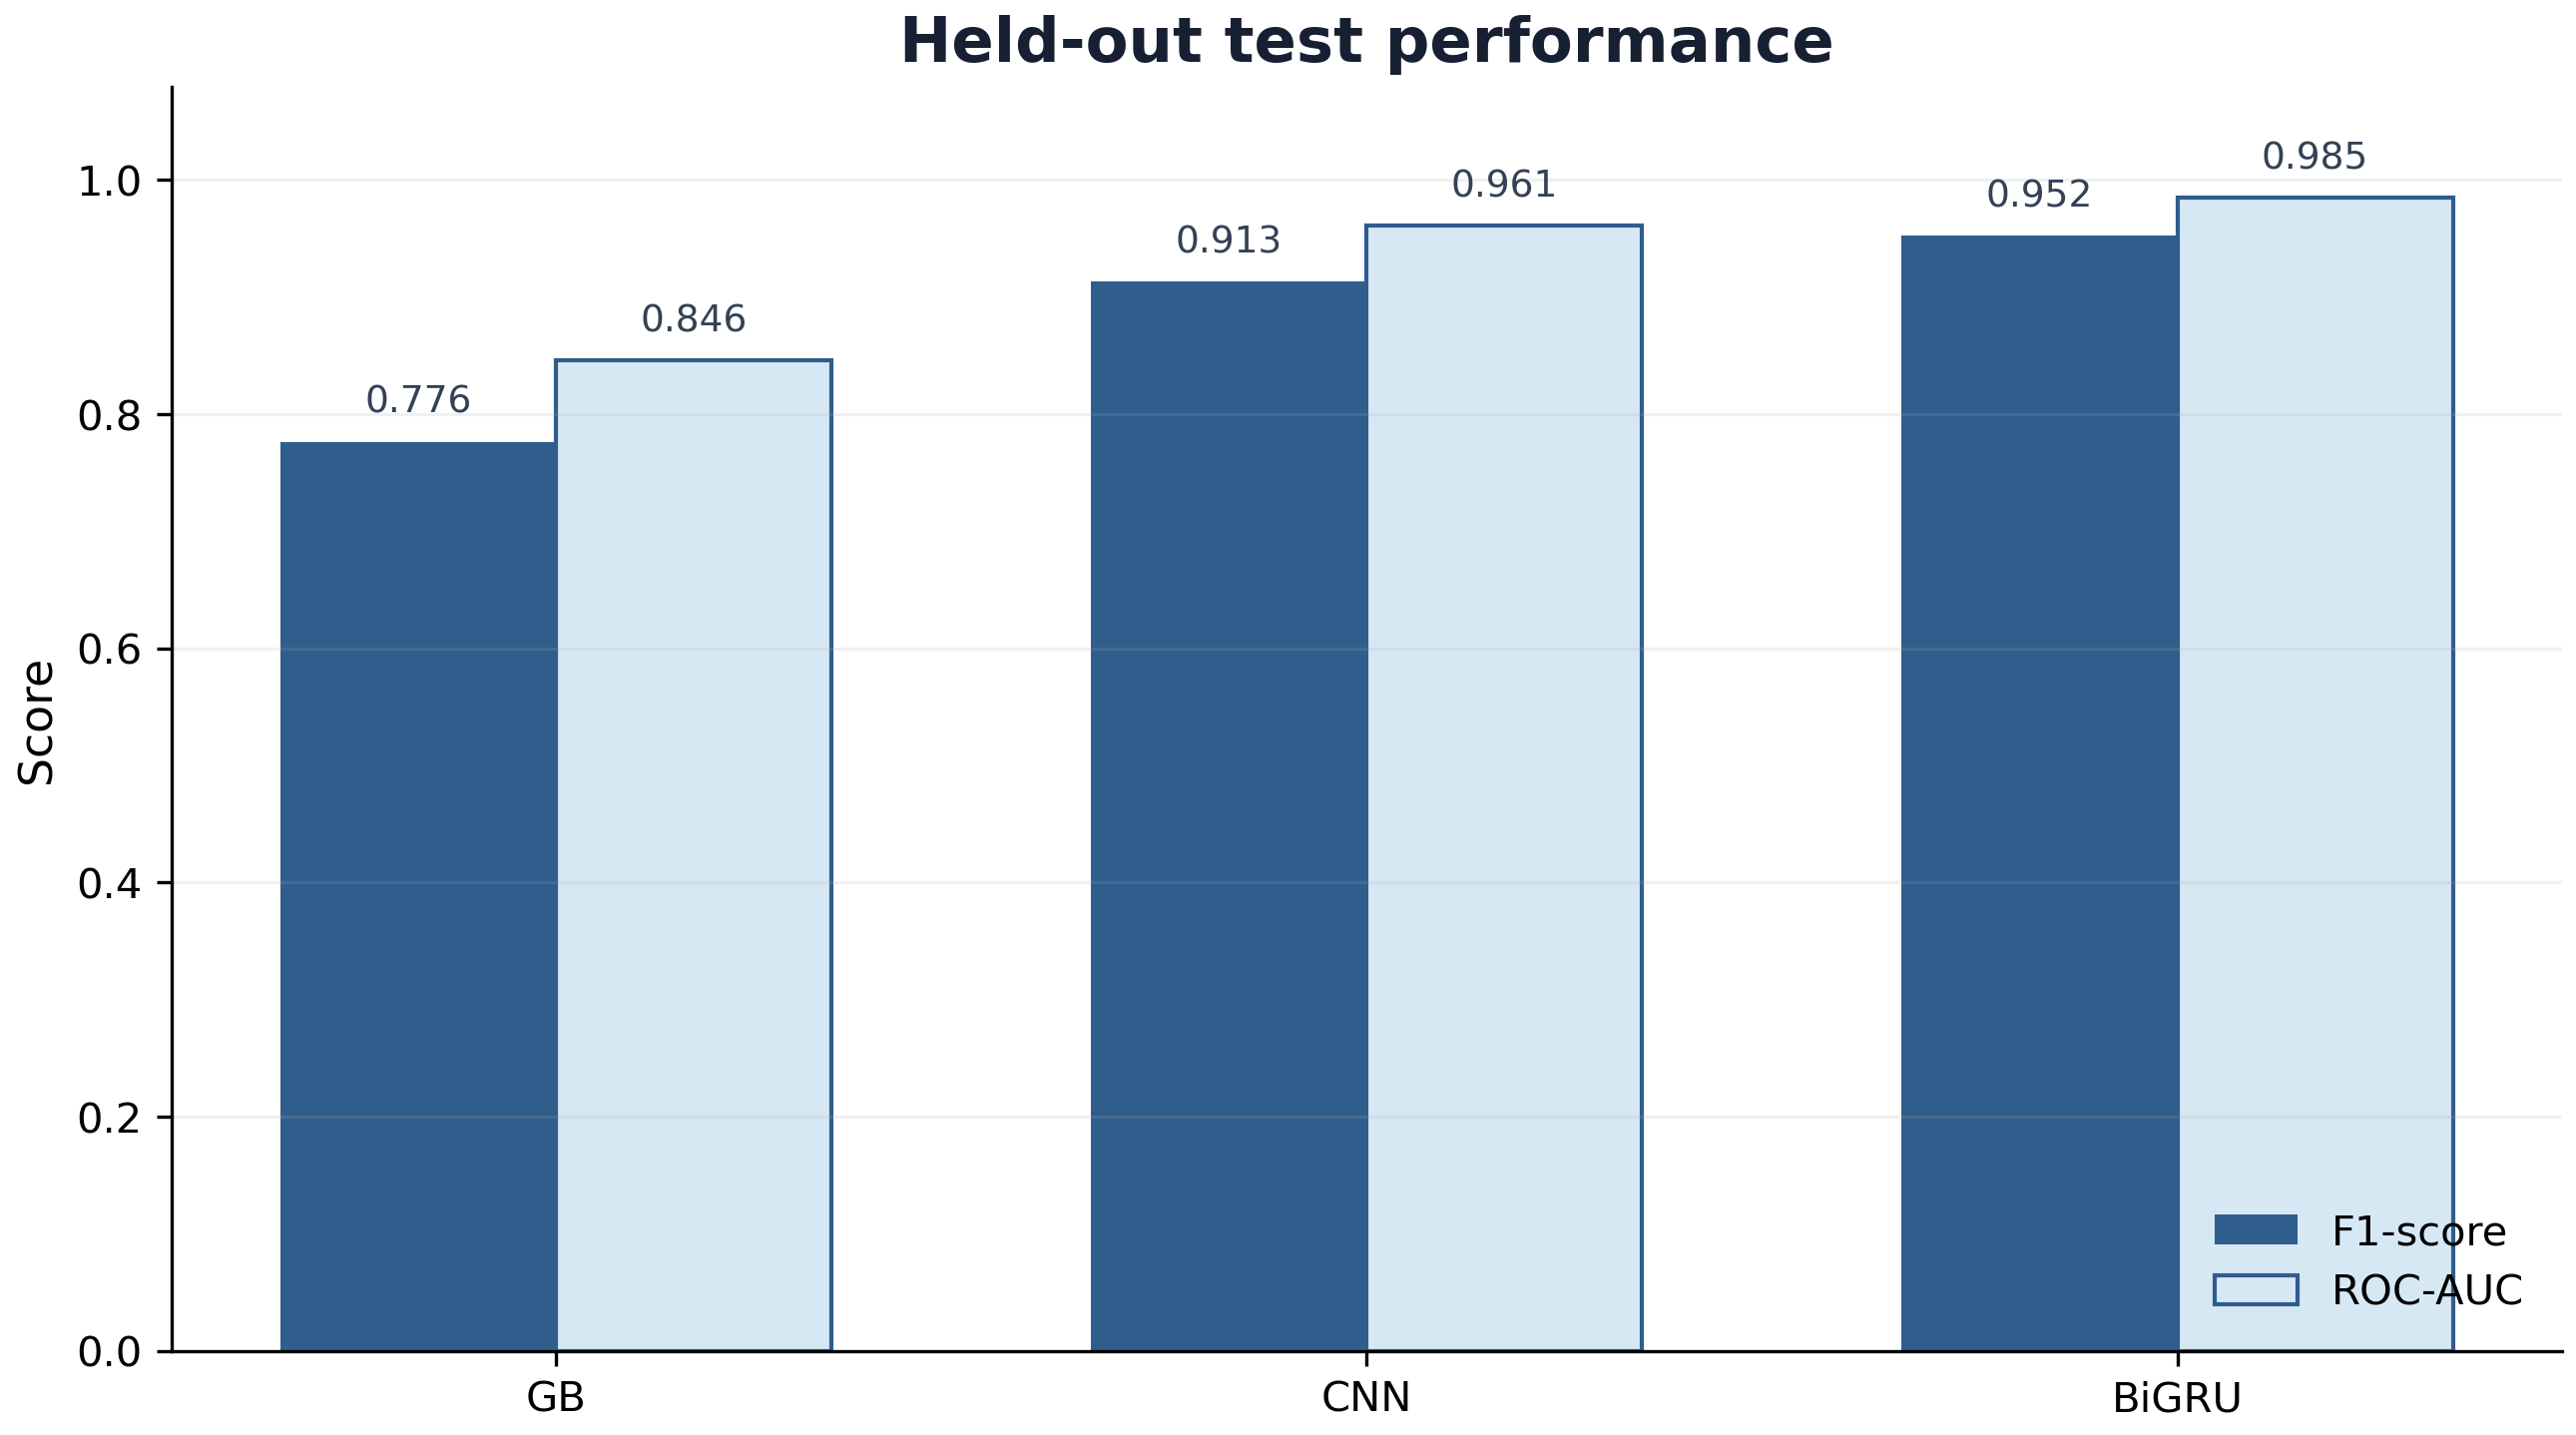
\includegraphics[width=0.72\linewidth]{figures/gb_cnn_rnn_compare.png}


\end{frame}

\begin{frame}{Classification performance}

\begin{table}
\centering
\small
\begin{tabular}{lccc}
\toprule
Model & F1-score & ROC--AUC & Runtime \\
\midrule
Gradient Boosting & 0.7765 & 0.8459 & 0.50 min \\
1D CNN & 0.9135 & 0.9607 & 1.39 min \\
BiGRU & 0.9523 & 0.9849 & 5.51 min \\
\bottomrule
\end{tabular}
\end{table}

\end{frame}

% -------------------------------------------------
% Slide 17: Model behavior
% -------------------------------------------------
\begin{frame}{Model behavior}

\begin{itemize}
    \item \textbf{Gradient Boosting} — Conservative filtering; higher read retention
    \item \textbf{CNN} — Sensitive model; more aggressive filtering
    \item \textbf{BiGRU} — Highest F1 score; best read-level performance
\end{itemize}

\end{frame}

% -------------------------------------------------
% Slide 18: Error patterns
% -------------------------------------------------
\begin{frame}{Error patterns}

\begin{columns}
\column{0.33\textwidth}
\centering
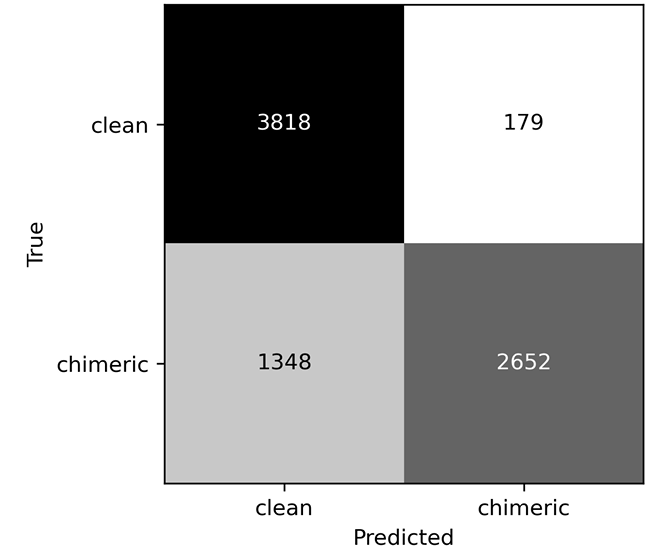
\includegraphics[width=0.90\linewidth]{figures/cm_gradient_boosting.png}\\
\small Gradient Boosting

\column{0.33\textwidth}
\centering
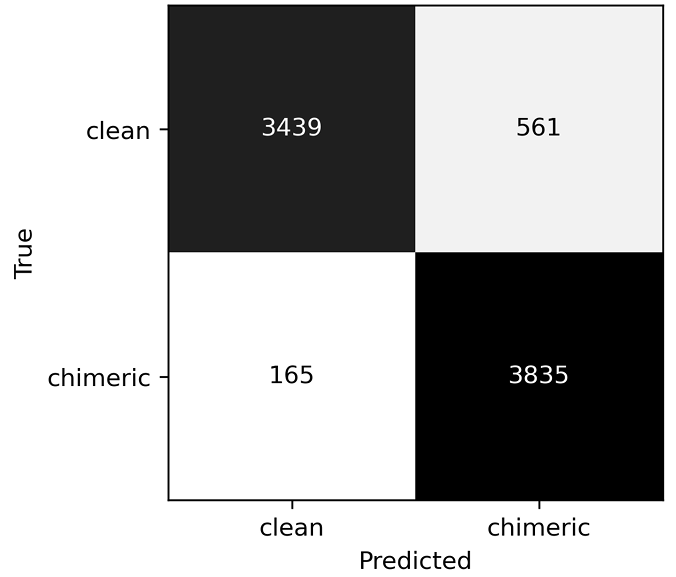
\includegraphics[width=0.90\linewidth]{figures/cnn_confusion.png}\\
\small CNN

\column{0.33\textwidth}
\centering
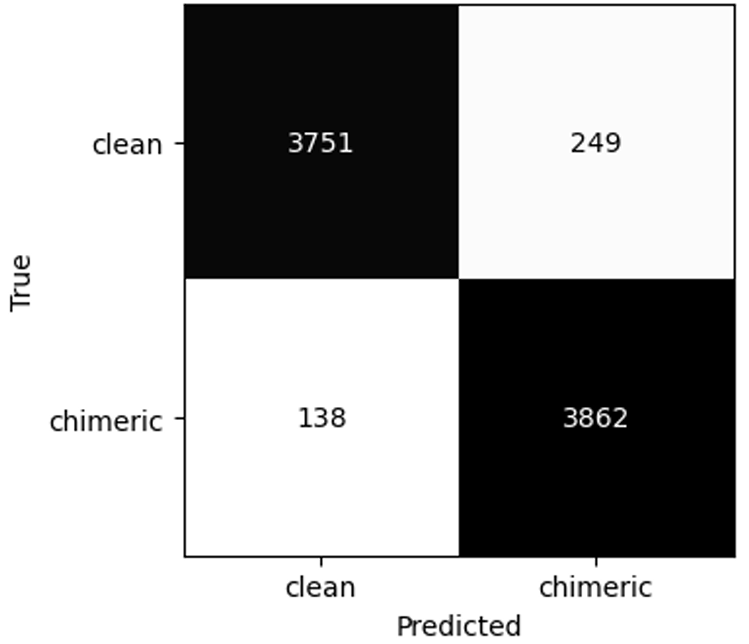
\includegraphics[width=0.90\linewidth]{figures/rnn_confusion.png}\\
\small BiGRU
\end{columns}


\end{frame}

% -------------------------------------------------
% Slide 19: Feature importance
% -------------------------------------------------
\begin{frame}{Feature importance}

\centering
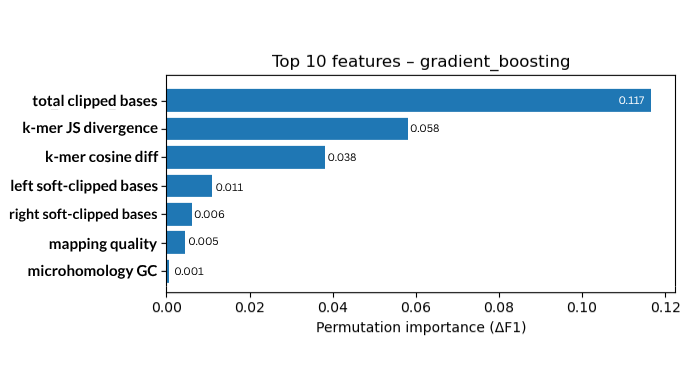
\includegraphics[
    width=\textwidth,
    height=0.72\textheight,
    keepaspectratio
]{figures/gradient_imp_pair.png}

\vspace{0.35em}

\begin{minipage}{0.96\textwidth}
\footnotesize
Most informative predictors: 
\textbf{total clipped bases}, 
\textbf{k-mer Jensen--Shannon divergence}, 
\textbf{k-mer cosine difference}, and 
\textbf{left soft clipping}.
\end{minipage}

\end{frame}

\begin{frame}{Feature Family Importance}

\begin{table}
\centering
\small
\begin{tabular}{lrrr}
\hline
\textbf{Family} & \textbf{Importance Sum} & \textbf{Importance Mean} & \textbf{nFeatures} \\
\hline
Clipping & 0.133830 & 0.033458 & 4 \\
K-mer jump & 0.096264 & 0.048132 & 2 \\
Other & 0.003676 & 0.001225 & 3 \\
Microhomology & 0.000347 & 0.000174 & 2 \\
SA structure & -0.000859 & -0.000066 & 13 \\
\hline
\end{tabular}
\end{table}

\end{frame}

% -------------------------------------------------
% Slide 20: Assembly validation high coverage
% -------------------------------------------------
\begin{frame}{Assembly validation: high coverage}

\begin{columns}
\column{0.58\textwidth}
\centering
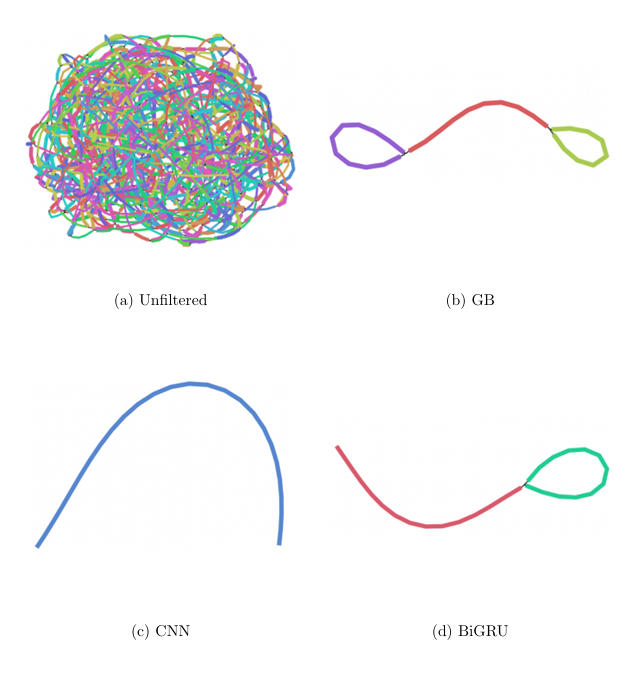
\includegraphics[width=0.80\linewidth]{figures/assembly_20k_50.png}

\column{0.38\textwidth}
\large
20K reads, 50\% chimeras

\vspace{0.7em}

\normalsize
\begin{itemize}
    \item Unfiltered assembly showed severe graph complexity.
    \item Filtering simplified the graph.
    \item CNN produced the simplest graph.
    \item GB retained more reads.
\end{itemize}
\end{columns}

\end{frame}

% -------------------------------------------------
% Slide 21: Assembly validation low coverage
% -------------------------------------------------
\begin{frame}{Assembly validation: low coverage}

\begin{columns}
\column{0.58\textwidth}
\centering
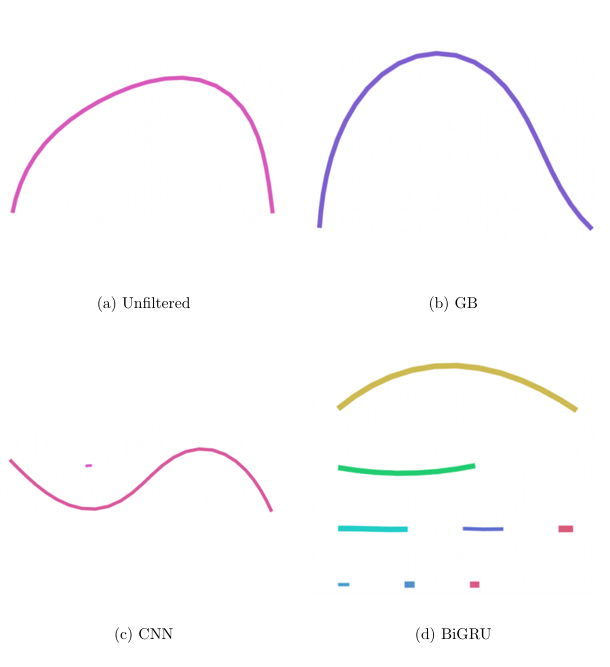
\includegraphics[width=0.80\linewidth]{figures/assembly_3200_50.png}

\column{0.38\textwidth}
\large
3,200 reads, 50\% chimeras

\vspace{0.7em}

\normalsize
At low read depth, aggressive filtering may remove too much read support and cause fragmentation.

\vspace{0.8em}

\begin{block}{Practical implication}
The safest model depends on coverage and chimera proportion.
\end{block}
\end{columns}

\end{frame}

% -------------------------------------------------
% Slide 22: Recommendations
% -------------------------------------------------
\begin{frame}{Recommendations: Practical Use}

\begin{itemize}
    \item Use \textbf{Gradient Boosting} when read depth is low.
    \item Use \textbf{BiGRU} when read-level classification is the priority.
    \item \textbf{CNN} may be useful in high-coverage and high-chimera conditions.
    
\end{itemize}

\end{frame}

\begin{frame}{Recommendations: Future Work}

\begin{itemize}
    \item Test on real mitochondrial datasets.
    \item Evaluate realistic class imbalance.
    \item Add varied sequencing-error profiles.
    \item Explore hybrid feature-sequence models.
\end{itemize}

\end{frame}

% -------------------------------------------------
% Slide 23: Summary
% -------------------------------------------------
\begin{frame}{Summary}

\large
\begin{enumerate}
    \item PCR-induced chimeras can disrupt mitochondrial genome assembly.
    \item Existing tools do not directly address this read-level setting.
    \item MitoChime detects suspected chimeric reads before assembly.
    \item BiGRU achieved the strongest classification performance.
    \item Model choice should consider both accuracy and read retention.
\end{enumerate}

\end{frame}

% -------------------------------------------------
% Slide 24: Final title
% -------------------------------------------------
{
\setbeamertemplate{footline}{}
\begin{frame}[plain]
\vspace{1.2cm}

\begin{center}
{\Huge \textbf{MitoChime}}\\[0.7em]

{\large A Machine Learning Pipeline for Detecting PCR-Induced}\\
{\large Chimeric Reads in Mitochondrial Illumina Data}\\[1.5em]

\rule{0.65\linewidth}{0.5pt}\\[1.2em]

{\normalsize
\presenters
}\\[1.5em]

{\large Thank you.}
\end{center}

\end{frame}
}

\end{document}